\cleardoublepage

\chapter{Badanie dużych modeli językowych w systemach RAG za pomocą autorskiego rozwiązania}

W tym rozdziale skupiono się na części praktycznej niniejszej pracy dyplomowej. Autor zaprezentował autorskie systemy RAG służące do testów dominujących dużych modeli językowych w zakresie odpowiadania na pytania dotyczące zewnętrznych nieustrukturyzowanych i ustrukturyzowanych źródeł danych. Badanie odbyło się 29 marca 2026 roku.


    \section{Cel badania}
    Celem badania było przetestowanie i porównanie pięciu popularnych i najnowszych dużych modeli językowych w zakresie trafności, kosztu, czasu i przepustowości tokenów generowanych odpowiedzi w oparciu o zewnętrzne źródła wiedzy. Były to następujące modele pięciu różnych liderów w zakresie GenAI: gpt-5-mini, deepseek-v3.2-exp, gemini-3-flash-preview, claude-haiku-4.5 i grok-4.1-fast. Do testów wykorzystano łącznie cztery ustrukturyzowane i nieustrukturyzowane zestawy danych. Wobec każdego z nich sformułowano 8 pytań z czterech kategorii. Każde pytanie zadano jednokrotnie dla każdej konfiguracji. Do stworzenia autorskich systemów RAG posłużyła platforma n8n \cite{n8n} stosowana do automatyzacji zadań i procesów. Po wykonanych testach, wykonano analizę wyników i wybrał optymalną konfigurację systemu.


    \section{Przygotowanie danych}
    Jako danych nieustrukturyzowanych użyto jedenastostronnicowego pliku PDF oraz pliku tekstowego. Oba odnosiły się do tego samego artykułu internetowego pt.: \enquote{Czym są duże modele językowe?} \cite{oracle_czym_sa_llm}. Pierwszy plik został stworzony poprzez bezpośrednie przekonwertowanie strony internetowej na PDF. Drugi plik powstał poprzez scraping treści z tej samej strony do formatu markdown, co później zostało zapisane do formatu .txt. Udało się to osiągnąć za pomocą platformy Firecrawl \cite{firecrawl}. Należy zaznaczyć, iż oba pliki w jednym miejscu zostały zmodyfikowane. Jedno z dwóch wystąpień roku \enquote{2017} zmieniono na \enquote{2002}. Modyfikacja ta została dokonana na potrzeby badania. Docelowo zawartości obu plików poddano procesowi wektoryzacji i zaindeksowania w bazie danych Pinecone \cite{pinecone}. Na poniższym rysunku \ref{vector_store_embedding_n8n} przedstawiono autorskie oprogramowanie wykonujące ten proces.

    \begin{center}
        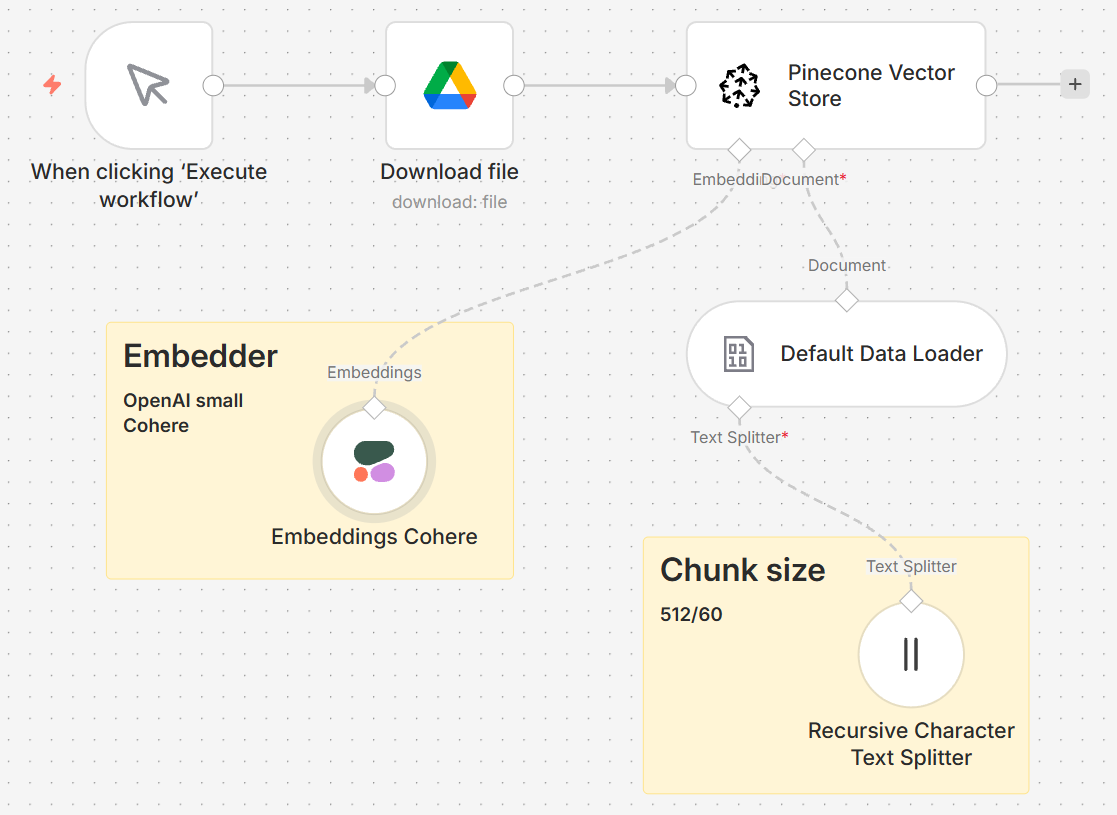
\includegraphics[width=0.5\textwidth]{rysunki/vector_store_embedding_n8n.png}
        \captionof{figure}{ Workflow w n8n służący do transformacji nieustrukturyzowanych danych w embeddingi zapisane do wektorowej bazy danych Pinecone \cite{n8n} }
        \label{vector_store_embedding_n8n}
    \end{center}

    \noindent W ramach przedstawionego workflow zastosowano segmentację tekstu (chunking) na fragmenty o długości 512 tokenów z marginesem części wspólnej (overlapping) wynoszącym 60 tokenów. Dla każdego z plików proces ten uruchomiono dwukrotnie, wykorzystując dwa różne modele osadzające: text-embedding-3-small od OpenAI (o wymiarowości 1536) oraz Embed-Multilingual-v3.0 od Cohere (o wymiarowości 1024). Dzięki temu, na platformie Pinecone przechowano cztery różne wektorowe bazy danych: pdf-openai, pdf-cohere, scraped-openai i scraped-cohere. Doskonale posłużyły one jako zewnętrzne źródła nieustrukturyzowanej wiedzy podczas testowania modeli w ramach systemów RAG.
    
    Jako źródło danych ustrukturyzowanych użyto bazę danych SQL i plik CSV. Oba zasoby zawierały takie same rekordy i zostały stworzone na podstawie ogólnodostępnego pliku products100.csv z repozytorium \enquote{sample-csv-files} na platformie GitHub \cite{products100_github}. Posiadał on 100 rekordów i następujące kolumny (atrybuty): Index, Name, Description, Brand, Category, Price, Currency, Stock, EAN, Color, Size, Availability, Internal\_ID. Do przechowania bazy SQL wykorzystano platformę Supabase \cite{supabase}, która działa w oparciu o system Postgres. Plik CSV znajdował się bezpośrednio na platformie n8n. Warto podkreślić, że żaden z plików nie został zmodyfikowany.


    \section{Przygotowanie pytań}
    Do testowania modeli językowych w dedykowanym systemie RAG autor utworzył dwa zestawy pytań \ref{pytania_nieustrukturyzowane} i \ref{pytania_ustrukturyzowane}. Pierwszy dotyczył danych nieustrukturyzowanych, a drugi danych ustrukturyzowanych. Podczas kreowania pytań zainspirowano się odpowiednimi artykułami naukowymi omawianymi w poprzednim rozdziale \cite{art2_unstructured2024} i \cite{art3_structured2024}.
        
    \begin{table}[h]
        \centering
        \caption{ Pytania do nieustrukturyzowanych źródeł danych }        
        \begin{tabularx}{\textwidth}{|l|X|}
        \hline
        \textbf{Kategoria} & \textbf{Pytanie} \\ \hline
        
        \multirow{4}{*}{Integracja informacji} & Jaki produkt firmy OpenAI jest powszechnie uważany za pierwszy współczesny model LLM i ile miał on parametrów? \\ \cline{2-2} 
         & Który model stworzony przez OpenAI uznaje się za pionierski w kategorii współczesnych LLM i jaka była skala jego parametrów? \\ \hline
        
        \multirow{4}{*}{Odporność na szum} & Jak automatyzacja z użyciem LLM wpływa na produktywność w komunikacji z klientami? \\ \cline{2-2} 
         & W jaki sposób wykorzystanie modeli językowych do automatyzacji przekłada się na efektywność obsługi klienta? \\ \hline
        
        \multirow{5}{*}{Odporność na błędne fakty} & W którym roku naukowcy z Google opublikowali artykuł wprowadzający architekturę Transformer? \\ \cline{2-2} 
         & Kiedy światło dzienne ujrzał przełomowy artykuł Google prezentujący nową architekturę, będącą fundamentem obecnego przełomu w generatywnej sztucznej inteligencji? \\ \hline
        
        \multirow{3}{*}{Odmowa odpowiedzi} & Kto jest szefem firmy OpenAI? \\ \cline{2-2} 
         & Na podstawie załączonego dokumentu wskaż, kto pełni funkcję dyrektora generalnego (CEO) firmy OpenAI. \\ \hline
        
        \end{tabularx}
        \label{pytania_nieustrukturyzowane}
    \end{table}

    Pierwszy zestaw pytań składał się z czterech kategorii: integracja informacji, odporność na szum, odporność na błędne fakty i odmowa odpowiedzi. Każda zawierała po dwa pytania dotyczące tej samej kwestii, jednak sformułowane na dwa różne sposoby. Łącznie było 8 pytań. Zgodnie z zewnętrznym źródłem wiedzy, odpowiedzi na pytania z każdej kategorii powinny odpowiednio przypominać poniższe, stanowiące punkt odniesienia:
    
    \begin{itemize}
        \item \enquote{\textit{Pierwszym współczesnym modelem LLM od firmy OpenAI był GPT-1 i posiadał on nieco ponad 100 milionów parametrów.}},
        
        \item \enquote{\textit{LLM znacząco podnosi produktywność w komunikacji z klientami: skracają czas oczekiwania i odciążają personel przez całodobowe, wielojęzyczne czatboty oraz automatyzację zadań follow‑up.  Istotnie wpływa na wzrost poziomu usług o 150\% i spadek kosztów o 30\%.}},
        
        \item \enquote{\textit{Artykuł Google wprowadzający architekturę Transormer ukazał się w 2017 roku. W jednym fragmencie dokumentu występuje błąd — podano tam 2002, a prawidłowy rok to 2017.}},
        
        \item \enquote{\textit{Niestety, nie umiem odpowiedzieć na to pytanie na podstawie dostępnego artykułu.}}.
    \end{itemize}

    \noindent Warto nadmienić, że w ramach niniejszego projektu, trzecia kategoria posłużyła sprawdzeniu czy LLM jest w stanie odpowiedzieć na złożone pytania wymuszające zebranie i połączenie ze sobą informacji z wielu sekcji (akapitów) pojedynczego dokumentu, a nie z wielu dokumentów. 

    \begin{table}[h]
        \centering
        \caption{ Pytania do ustrukturyzowanych źródeł danych }        
        \begin{tabularx}{\textwidth}{|l|X|}
        \hline
        \textbf{Kategoria} & \textbf{Pytanie} \\ \hline
        
        \multirow{2}{*}{Łatwe} & Ile produktów jest w bazie? \\ \cline{2-2} 
         & Ile kosztuje rower? \\ \hline
        
        \multirow{2}{*}{Umiarkowane} & Które produkty kosztują więcej niż 920 USD? \\ \cline{2-2} 
         & Wypisz produkty, których 'Internal\_ID' wynosi 3. \\ \hline
        
        \multirow{3}{*}{Trudne} & Ile łącznie kosztują produkty: Smart Lamp, Eco Radio i Fast Keyboard? \\ \cline{2-2} 
         & Jaka jest łączna wartość magazynowa (Price × Stock) produktów dostępnych jako 'out\_of\_stock'? \\ \hline

         \multirow{3}{*}{Odmowa odpowiedzi} & Jaki kolor ma krzesło? \\ \cline{2-2} 
         & Na podstawie tabeli, wskaż na który produkt czas oczekiwania jest najdłuższy. \\ \hline
        
        \end{tabularx}
        \label{pytania_ustrukturyzowane}
    \end{table}

    Drugi zestaw pytań także składał się z czterech kategorii: łatwe, umiarkowane, trudne i odmowa odpowiedzi. Każda zawierała po dwa różne pytania. Łącznie było 8 zapytań. Zgodnie z zewnętrznym źródłem wiedzy, odpowiedzi na wszystkie osiem pytań powinny w odpowiedni sposób nawiązywać do poniższych przykładów, stanowiących punkt odniesienia:

    \begin{itemize}
        \item \enquote{\textit{W bazie jest 100 produktów.}},
        
        \item \enquote{\textit{Rower kosztuje 234 USD.}},
        
        \item \enquote{\textit{Jest 6 produktów kosztujących więcej niż 920 USD: Ultra Speakerphone Oven Go Smart, Fast Keyboard, Clock Brush, Eco Iron Monitor Air, Fast Fan i Rechargeable Projector.}},
        
        \item \enquote{\textit{Znaleziono 2 produkty o Internal\_ID równym 3: Smart Webcam Projector Lock i Smart Lamp}},

        \item \enquote{\textit{Łączny koszt produktów Smart Lamp, Eco Radio i Fast Keyboard wynosi 1523 USD.}},
        
        \item \enquote{\textit{Łączna wartość magazynowa produktów o statusie 'out\_of\_stock' wynosi 3 219 633 USD.}},
        
        \item \enquote{\textit{Niestety, nie umiem odpowiedzieć na to pytanie na podstawie dostępnej bazy danych.}},
        
        \item \enquote{\textit{Niestety, nie umiem odpowiedzieć na to pytanie na podstawie dostępnej bazy danych.}}.
    \end{itemize}
    
    
    \section{Przeprowadzenie testów}
    W celu przeprowadzenia testów utworzono trzy scenariusze automatyzacji testów (workflow) na platformie n8n, które przedstawiono na rysunkach \ref{mgr_unstructured_structuredSQL_n8n} i \ref{mgr_structured_csv_n8n}. Każdy z nich działał w zbliżony sposób, a jedyną różnicę stanowiły narzędzia agentów AI oraz wiadomości systemowe, które znajdują się w dołączonym do pracy pliku ZIP oraz w repozytorium plików autora na platformie GitHub \cite{moje_repozytorium}. W pierwszej kolejności należało podać prompt (zapytanie), które następnie zostało przekazane do pięciu agentów AI. Każdy z nich miał dołączony odpowiedni model, do którego dostęp zapewniało API programu OpenRouter \cite{openrouter}. Agenty AI były połączone z zewnętrznymi źródłami danych dzięki odpowiednim narzędziom, które zdefiniowano w późniejszej części bieżącej sekcji. Odpowiedzi dużych modeli językowych na zadane pytania gromadziły się następnie w węźle Merge. Tak zestawione wyniki zostały automatycznie wpisane do odpowiedniej kolumny w dedykowanym arkuszu Google. Liczbę tokenów oraz czas generowania odpowiedzi spisywano ręcznie z parametrów agentów po każdym wykonanym teście do tego samego arkusza.

    \begin{center}
        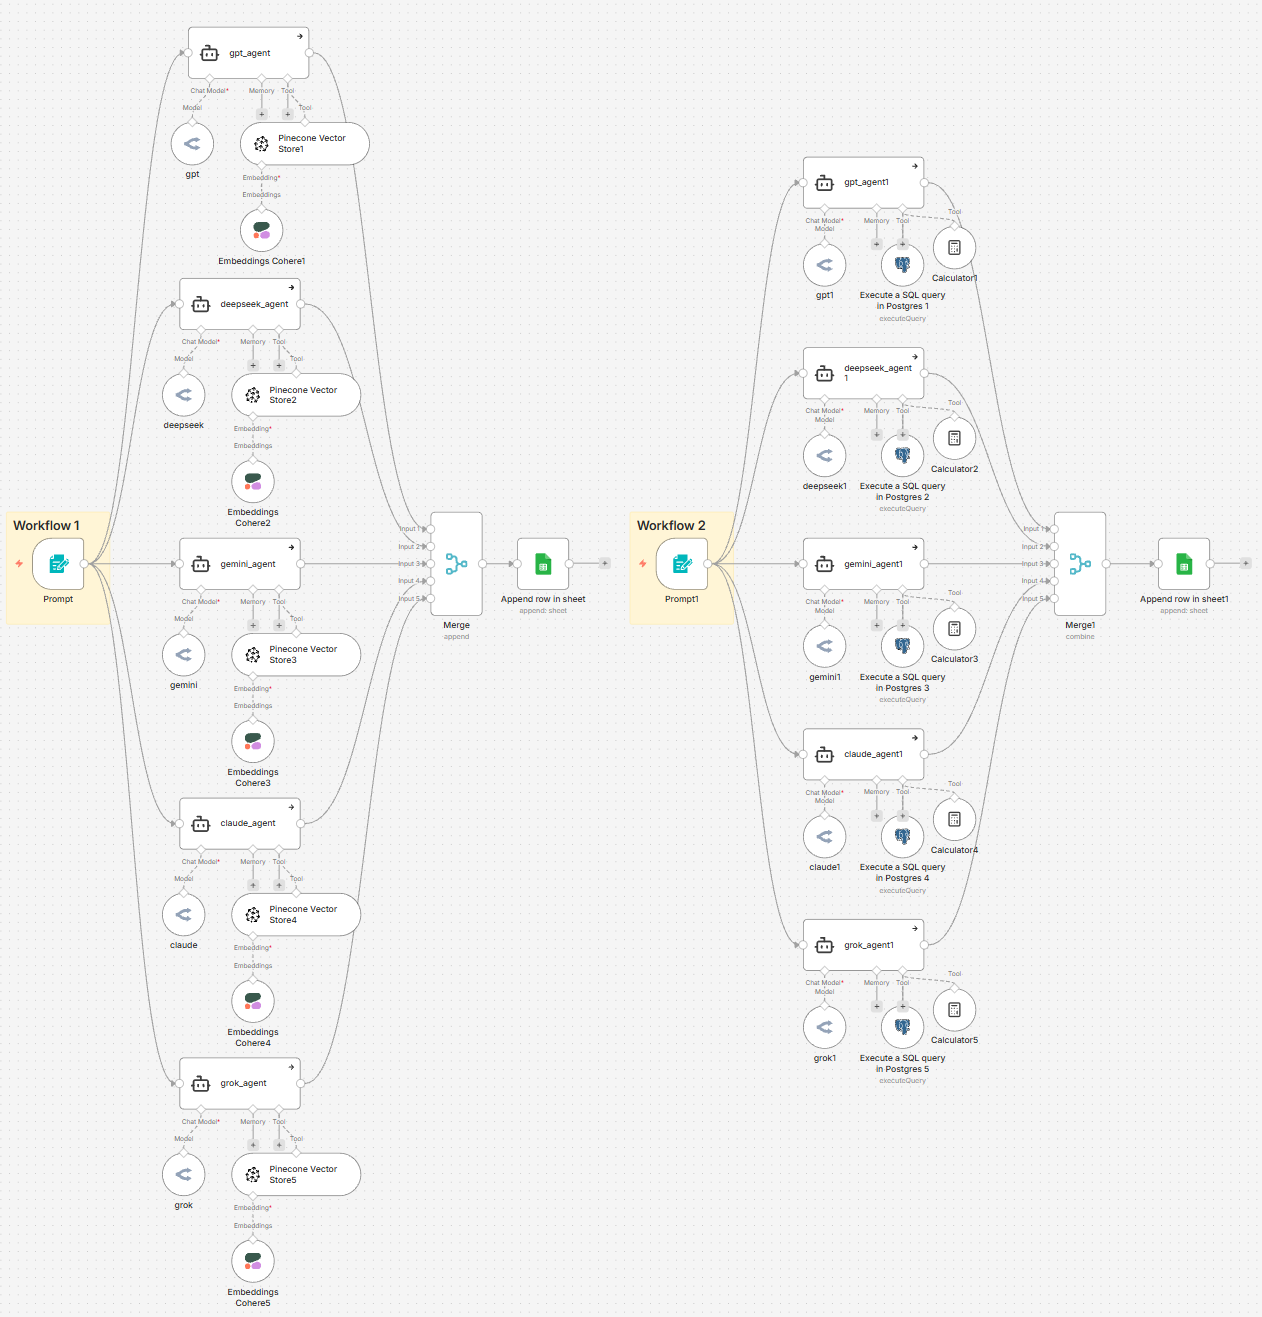
\includegraphics[width=0.8\textwidth]{rysunki/mgr_unstructured_structuredSQL_n8n.png}
        \captionof{figure}{ Dwa scenariusze automatyzacji testów systemów RAG — Workflow 1 dla dokumentu PDF i pliku tekstowego oraz Workflow 2 dla bazy danych SQL \cite{n8n}}
        \label{mgr_unstructured_structuredSQL_n8n}
    \end{center}

    W pierwszym workflow, do zewnętrznego źródła danych można było się odnieść za pomocą narzędzia dedykowanego wektorowym bazom danych Pinecone. W opisie narzędzia zawarto taką treść: \enquote{\textit{Użyj tego narzędzia, aby przeszukać bazę wektorową zawierającą treść artykułu firmy Oracle o dużych modelach językowych}}. W zależności od tego jaki embedder został użyty do utworzenia konkretnej bazy wektorowej, taki też był stosowany w danym przypadku do wydobywania niezbędnych informacji.
    
    W drugim workflow, do zewnętrznej bazy danych SQL można było się odnieść za pomocą narzędzia Postgres. Umożliwiło ono ekstrakcję danych stosując wygenerowane zapytanie w formacie SQL przez duży model językowy, aby poprawnie odpowiedzieć na zadane przez użytkownika pytanie. Dodatkowym narzędziem był kalkulator. Ułatwił on wykonywanie skomplikowanych obliczeń matematycznych, z którymi LLMy w takiej konfiguracji mają sporo trudności.

    \begin{center}
        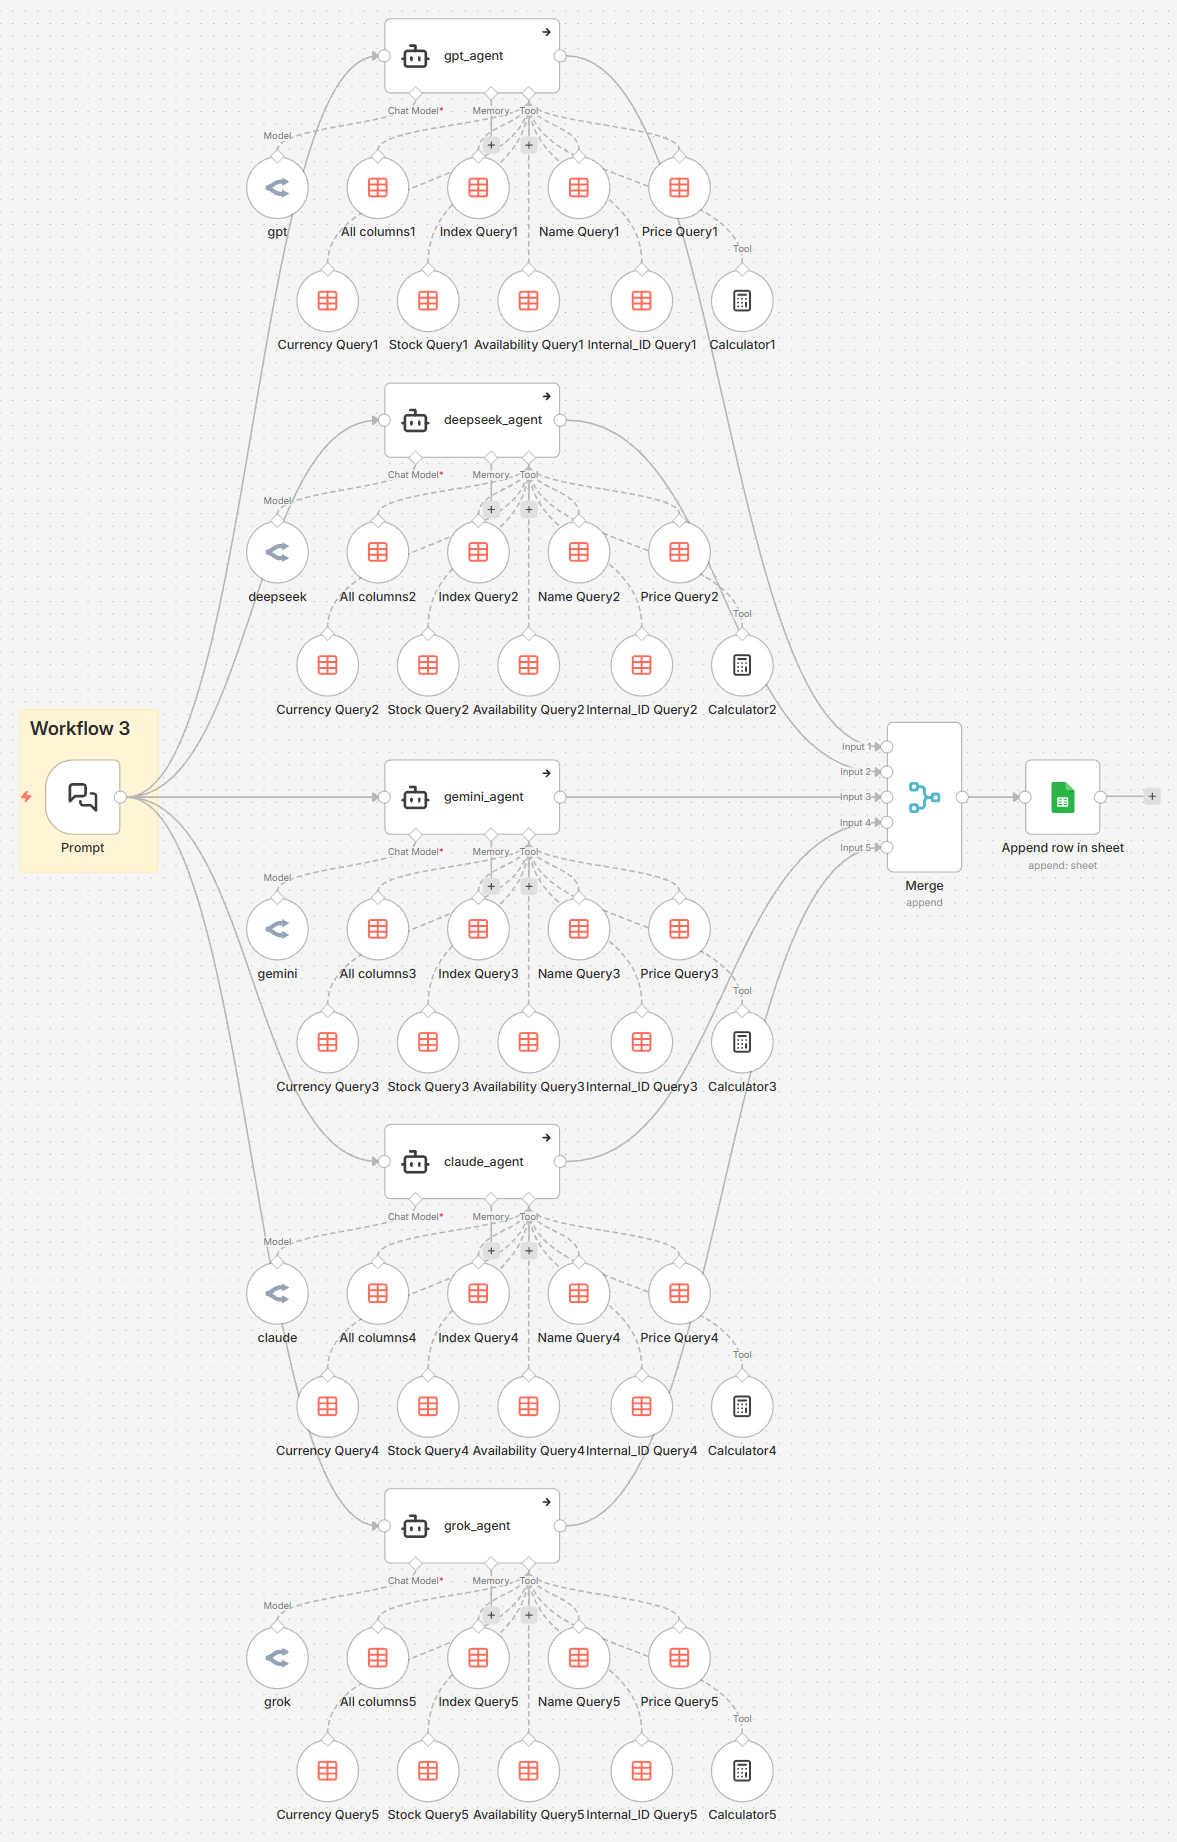
\includegraphics[width=0.6\textwidth]{rysunki/mgr_structured_csv_n8n.png}
        \captionof{figure}{ Scenariusz automatyzacji testów systemów RAG — Workflow 3 dla pliku CSV \cite{n8n}}
        \label{mgr_structured_csv_n8n}
    \end{center}

    W trzecim workflow wydobycie informacji z pliku CSV przechowywanego na tej samej platformie było bardziej skomplikowane. Należało użyć węzłów Data Table Tool, które służyły do wydobycia informacji z konkretnych kolumn pliku. W ramach tego badania, były to tylko kolumny zawierające dane niezbędne do odpowiedzi na zadawane pytania. Podobnie jak w drugim workflow, tutaj także agenty AI korzystały z kalkulatora.

    W ramach powyższych scenariuszy testowych powstało łącznie 30 różnych konfiguracji systemów RAG, po sześć dla każdego badanego modelu LLM. Tabela poniżej \ref{systemy_rag} prezentuje podział i nazwy tych systemów dla wybranych modeli.

    \begin{table}[H]
        \centering
        \caption{ Wykaz 30 implementacji systemów RAG stworzonych dla pięciu wybranych modeli LLM }
        \begin{tabularx}{\textwidth}{|p{4cm}|X|}
        \hline
        \textbf{Model LLM} & \textbf{Dedykowane systemy RAG} \\
        \hline
        gpt-5-mini &  gpt-pdf-openai, gpt-pdf-cohere, gpt-scraped-openai, gpt-scraped-cohere, gpt-sql, gpt-csv \\ \hline
        
        deepseek-v3.2-exp &  deepseek-pdf-openai, deepseek-pdf-cohere, deepseek-scraped-openai, deepseek-scraped-cohere, deepseek-sql, deepseek-csv \\ \hline
        
        gemini-3-flash-preview  &  gemini-pdf-openai, gemini-pdf-cohere, gemini-scraped-openai, gemini-scraped-cohere, gemini-sql, gemini-csv \\ \hline

        claude-haiku-4.5 &  claude-pdf-openai, claude-pdf-cohere, claude-scraped-openai, claude-scraped-cohere, claude-sql, claude-csv \\ \hline

        grok-4.1-fast &  grok-pdf-openai, grok-pdf-cohere, grok-scraped-openai, grok-scraped-cohere, grok-sql, grok-csv \\ \hline
        \end{tabularx}
        \label{systemy_rag}
    \end{table}

    